\documentclass[]{article}
\usepackage[version=3]{mhchem}
\usepackage{natbib}
\usepackage{graphicx}
\usepackage{float}
\bibliographystyle{abbrvnat}
\usepackage[colorlinks]{hyperref}
\hypersetup{
  citecolor = {blue},
}
\newcommand{\unit}[1]{\ensuremath{\, \mathrm{#1}}}

\title {Procedimiento experimental para determinar el potencial bioquímico de metano utilizando el método basado en la densidad del biogás\footnote{
  Citación recomendada: 
Hafner, S.D.; Astals, S.; Holliger, C.; Justesen, C.; Koch, K.; Mortensen, J.R. 2021 Gas density-based BMP measurement. Standard BMP Methods document 304, version 2.1. Available online: https://www.dbfz.de/en/BMP (accessed on March 31, 2021).
\newline
  En \url{https://www.dbfz.de/en/BMP} encontraréis un documento BibTeX para importarlo al gestor de referencias.
\newline
  Este documento es una traducción al español realizada por Sergi Astals y Glen B. Madrigal del documento original en inglés (versión 2.1). En caso de duda el documento en inglés prevalece sobre esta traducción.
}
}
\author{Sergi Astals, Sasha D. Hafner, Christof Holliger, \\ Camilla Justesen, Konrad Koch, Jacob R. Mortensen, \\ S\"oren Weinrich 
\\
\texttt{sastals@ub.edu}\\
}

\date{\today \\
\bigskip
\textit{
  Documento número 304.
  Versión en español 2.0.
    Este documento forma parte de una serie de documentos dedicados a la estandarización de los ensayos de medición del potencial bioquímico de metano.\footnote{Para más información y otros documentos visite \url{https://www.dbfz.de/en/BMP}. 
    Para ver el historial de versiones y proponer cambios visite \url{https://github.com/sashahafner/BMP-methods}.}
}
}

\begin{document}
\maketitle

\section{Introducción}
El método para medir el potencial bioquímico de metano utilizando la densidad del biogás (GD-BMP del inglés \textit{gas-density biochemical methane potential}) tiene la ventaja de utilizar materiales disponibles en la mayoría de laboratorios y ser de bajo costo. 
El método GD-BMP utiliza la pérdida de masa y el volumen de biogás venteado de uno o más intervalos para determinar la densidad del biogás y, con ello, su composición.\footnote{La composición solo se puede determinar a partir de la densidad cuando la mezcla contine dos gases, \ce{CH4} y \ce{CO2} en nuestro caso.}
Una vez calculada la densidad del biogás, la producción de metano (\ce{CH4}) se puede calcular con el volumen de biogás venteado o con la pérdida de masa de la botella. 
Este documento describe el procedimiento experimental para realizar el método GD-BMP en el laboratorio.
El desarrollo y validación del método GD-BMP está explicado en \citet{justesenDevelopmentValidationLowcost2019}, documento de acceso abierto. El documento 204 de esta colección de documentos explica detallamente los cálculos para el método GD-BMP e incluye un ejemplo \citep{BMPdoc204gasdens}. 

\section{Material necesario}
\label{sec:equipment}
Para realizar el método GD-BMP se necesitan los siguientes materiales:
\begin{itemize}
    \item Balanza de laboratorio
    \item Jeringa y agujas
    \item Manómetro
    \item Botellas y septos
    \item Incubatora
\end{itemize}

La precisión de la balanza dependerá de la cantidad de biogás que se va a producir. La precisión mínima\footnote{
  Los proveedores normalmente reportan la precisión de una balanza como ``linealidad''. 
  Recalcar que precisión no es lo mismo que ``legibilidad'', que es la masa mínima que puede leer la balanza. 
} requerida para la balanza es de 30 mg por cada gramo de sólido volátil (SV) de sustrato utilizado.\footnote{
  Por ejemplo, si se añaden 2 gramos de SV de sustrato a cada botella, la precisión de la balanza tiene que ser 60 mg o superior (p.ej. 50 mg sería suficiente).
}
Como se explica posteriormente, comprobar la precisión y estabilidad de la balanza forma parte del procedimiento experimental.

Un manómetro cerrado en forma de U\footnote{
  Este manómetro puede hacerse con un tubo de plástico con agua. Para cerrar el tubo se puede usar una válvula o, simplemente, doblando el tubo y una pinza. Ver Fig. \ref{fig:utube} a modo de ejemplo.  
} o un manómetro digital sencillo es suficiente para verificar que la presión del espacio de cabeza después del venteo es la atmosférica.

Lo ideal es tener jeringas con volumenes diferentes para tener una buena precisión en producciones altas y bajas de biogás. Idealmente, la jeringa de mayor volumen debería ser suficientemente grande para contener todo el biogás producido en un intervalo de medición.\footnote{
\label{fn:cellrate}
  La velocidad de producción de biogás depende de las propiedades del sustrato y el inóculo. La mejor forma de estimarlo es utilizando datos de experimentos previos.
  Para la celulosa microcristalina, la velocidad máxima de producción de biogás es, aproximadamente, 200 mL g$^{-1}$ d$^{-1}$ (por gramo de SV) durante los primeros días, aunque se han observado valores superiores a 300 mL g$^{-1}$ d$^{-1}$ \citep{hafnerImprovingInterlaboratoryReproducibility2020}.
  Para 2 gramos de SV de sustrato, el volumen de la jeringa tendría que ser superior a 600 mL (300 $\times$ 2), pero se puede utilizar una jeringa de menor volumen (100 mL) realizando varios ciclos (ver Sección \ref{sec:volmeas}).
}
Pero las jeringas grandes son caras. Alternativamente, se puede utilizar una jeringa de menor volumen realizando varios ciclos para extraer todo el biogás producido en un intervalo de medición.
Sin embargo, esta estrategia de muestreo requiere una válvula y complica ligeramente el pocedimiento experimental (ver Sección \ref{sec:volmeas}).

Una incubadora o una sala de temperatura controlada es necesaria para mantener las botellas a la temperatura de ensayo (p.ej. 37 $^\circ$C).
Utilizar un baño de agua no es recomendable, ya que el agua en la superficie de la botella afectará la masa de la botella y los resultados.
Idealmente, el venteo y pesado de las botellas debería realizarse dentro de una sala de temperatura controlada, de esta forma las botellas y el espacio de cabeza siempre estarían a la temperatura de ensayo (valores necesarios para los cálculos).
Sin embargo, el impacto de la temperatura del espacio de cabeza en los resultados es pequeño, por lo que no es estrictamente necesario.
No hace falta agitar constantemente las botellas con un agitador orbital o similares. Se ha observado que agitar suavemente las botellas antes del muestreo es suficiente (ver Sección \ref{sec:incsam}).\footnote{Se pueden agitar suavemente las botellas constantemente o intermitentemente con un agitador orbital, siempre y cuando el líquido no toque el septo.}

\section{Preparación}
\label{sec:setup}
Durante la preparación, el sustrato y el inóculo se añaden a la botella. Posteriormente, se lava el espacio de cabeza de la botella con \ce{N2} para eliminar el \ce{O2} y asegurar condiciones anaeróbicas. Finalmente, se pesan las botellas y se ponen en la incubadora.
La preparación del experimento debería considerar los requisitos mínimos detallados en el documento 100 \citep{BMPdoc100req}, incluyendo el control positivo de celulosa microcristalina\footnote{La celulosa microcristalina es el control positivo recomendado, aunque otros sustratos pueden utilizarse si no se tiene acceso a ella (ver \citet{kochEvaluationCommonSupermarket2020}).} y realizar todos los ensayos, como mínimo, por triplicado.

\subsection{Cantidad de inóculo y sustrato, y tamaño de botella}
\label{sec:quantities}
Dedicir la cantidad de inóculo y sustrato, y el tamaño de la botella necesario se realiza, generalmente, mediante experiencias previas. A continuación se detallan unas pautas generales, aunque estos valores pueden ajustarse en función de resultados previos y las caracteristicas del sustrato. 

El método GD-BMP requiere determinar pequeñas pérdidas de masa de botellas mayor masa y, consecuentemente, se intenta promover pedidas de masa elevadas.
Se recomienda que la cantidad de sustrato en cada botella sea, como mínimo, de 1 gramo de  SV.
Teniendo en cuenta este valor, la cantidad de inóculo se determina utilizando la relación inóculo:sustrato (RIS) (en ingles ISR de \textit{inoculum to substrate ratio}). La RIS más utilizada es 2:1 y se calcula en unidades de SV.\footnote{Ver \citet{holligerStandardizationBiomethanePotential2016} para más información.}

Una vez determinada la candidad de sustrato e inóculo, se puede determinar el tamaño de la botella. Alternativamente, para un determinado volumen de botella, se puede calcular la cantidad necesaria de sustrato e inóculo. Mencionar que los resultados del método GD-BMP no están muy afectados por la presión del espacio de cabeza y, además, el método permite corregir por fugas de biogás.
Sin embargo, por razones de seguridad (explosiones) y para evitar otros problemas (p.ej. excesiva disolución de \ce{CO2}), la presión del espacio de cabeza no debería superar los 200 kPa (2 bar) de sobrepresión, o mejor, 100 kPa \citep{hafnerSystematicErrorManometric2019}. 
La presión del espacio de cabeza se puede estimar mediante el volumen del espacio de cabeza y la producción de biogás esperada.
El volumen del espacio de cabeza se puede estimar asumiendo una densidad de 1 mL g$^{-1}$ para la mezcla de sustrato e inóculo. Para evitar el contacto entre el líquido y el septo (por espumas o durante la agitación) se recominenda que las botellas no se llenen más de un 50\%.

Utilizando los datos de la nota \ref{fn:cellrate} para la celulosa microcristalina (producción máxima de biogás de 200 mL g$^{-1}$ d$^{-1}$ pero de hasta 300 mL g$^{-1}$ d$^{-1}$) y la presión máxima recomendada del espacio de cabeza, el volumen del espacio de cabeza debe ser entre 100 y 300 mL por gramo SV de sustrato. 
El volumen del espacio de cabeza puede ser ajustado teniendo en cuenta la velocidad de degradación y el potencial de biometanización del sustrato respecto a la celulosa.

La diferencia de densidad entre el \ce{N2} (gas de lavado) y el biogás es una fuente de error, sobre todo al inicio del experimento. Aunque este error se puede corregir \citep{justesenDevelopmentValidationLowcost2019}, esta fuente de error se puede minimizar diminuyendo la relación entre el espacio de cabeza y el volumen de líquido. Por esto, no se recomiendan volumenes del espacio de cabeza superiores a 300 mL g$^{-1}$ (especialmente para el inóculo y sustratos lentamente biodegradables).

La herramienta ``Plan BMP'' en la aplicación OBA (online y gratuita) ayuda a calcular la cantidad de sustrato e inóculo \url{https://biotransformers.shinyapps.io/oba1/}.
Esta herramienta también comprueba valores de sustrato e inóculo respecto a los recomendados en  \citet{holligerStandardizationBiomethanePotential2016}.
La Tabla \ref{tab:examples} muestra tres ejemplos de preparación del ensayo GD-BMP para diferentes volúmenes de botella. Los tres ejemplos cumplen los requisitos mínimos de \citet{holligerStandardizationBiomethanePotential2016} y las recomendaciones específicas del método GD-BMP.

\begin{table}[h] 
\centering
\caption{Ejemplo de preparación de las botellas para el método GD-BMP.}
\label{tab:examples}
\begin{tabular}{llll}
\hline
Parámetro                     & A    & B   & C   \\
\hline
Volumen botella (mL)      & 520  & 250 & 160 \\
Inóculo SV (\% base húmeda)           & 2.0  & 2.0 & 4.0 \\
Sustrato VS (\% base húmeda)          & 99   & 99  & 99  \\
RIS (en SV)                & 2.0  & 2.0 & 2.0 \\
Sustrato SV (g)              & 1.50 & 1.0 & 1.0 \\
Cantidad de inóculo (g)               & 150  & 101 & 50  \\
Cantidad de sustrato (g)              & 1.52 & 1.0 & 1.0 \\
Cantidad de la mezcla (g)                & 152  & 101 & 51  \\
Espacio de cabeza (mL)         & 368  & 149 & 109 \\
Espacio de cabeza:sustrato SV (mL:g) & 245  & 149 & 109 \\
\hline
\end{tabular}
\end{table}

\subsection{Instrucciones paso a paso}
\begin{enumerate}
  \item Nivelar la balanza en una superficie estable (de acuerdo con las intrucciones del fabricante) y comprobar la precisión de la balanza con un juego de pesas.
      Es importante que la precisión de la balanza sea similar a la reportada, especialmente cuando se pesa un objeto de masa parecida al de las botellas de ensayo. Por ejemplo, para una balanza con una precisión de 50 mg esto se puede verificar tarando la balanza con una botella con agua y añadiendo un peso de 50 mg. Problemas de precision y estabilidad suelen ser causados por suciedad o corrientes de aire. Estos problemas se pueden solucionar limpiando y cambiando de lugar la balanza o bloqueando las corrientes de aire (p.ej. con una caja de cartón).
    \item Añadir la candidad de sustrato, inóculo y otros (p.ej. solución de micronutrientes \citep{holligerStandardizationBiomethanePotential2016}) a cada botella, sellar con un septo y asegurarlo. Se recomienda medir por peso la cantidad de sustrato e inóculo añadida a cada botella: tarar la balanza con la botella, añadir aproximadamente la cantidad deseada, limpiar el material que quede cerca de la boca de la botella y, finalmente, anotar la cantidad exacta añadida. La balanza utilizada para preparar las botellas no tiene porque ser la misma balanza que se utilice para monitorear los ensayos (ver Sección \ref{sec:incsam}).
    \item Lavar el espacio de cabeza para eliminar el \ce{O2}. 
    Una opción es pinchar el septo con una aguja que este conectada a una fuente de \ce{N2} (p.ej. red de gas
    del laboratorio, cilindro de \ce{N2}) mediante un tubo de plástico. Para evitar presiones elevadas es importante que haya un rotámetro entre la fuente de nitrógeno y la botella. Una segunda aguja es necesaria para dejar salir el nitrógeno de la botella. Para el método GD-BMP, es preferible lavar el espacio de cabeza con \ce{N2} en contraposición a una mezcla de \ce{N2} y \ce{CO2}.\footnote{Lavar el espacio de cabeza con \ce{N2} ocasiona pequeños errores en los resultados debido a diferencia de densidad entre el \ce{N2} y el biogás producido (la densidad del \ce{N2} es idéntica a la de un biogás con una mezcla \ce{CH4}:\ce{CO2} del 58\% de \ce{CH4}). En la mayoria de casos, esta fuente de error es despreciable pero existe la opción de corregir los cálculos \citep{justesenDevelopmentValidationLowcost2019}.
} 
      Evitar que el gas de lavado entre en contacto con el líquido de la botella (no burbugear para evitar el stripping de \ce{CO2}).
      Minimizar el stripping de \ce{CO2} utilizando un tiempo de lavado que solo renueve el volumen del espacio de cabeza 3 o 4 veces.
      Una vez transcurrido este tiempo, sacar la jeringa de entrada. Después de 2 segundos (para equilibrar la presión del espacio de cabeza con la atmosférica) quitar la otra jeringa.
      
     \item Añadir 3 botellas de ``control'' para verificar la estabilidad de la balanza.
      Es importante que estas botellas tengan peso contante durante todo el ensayo. 
      Idealmente deberían tener el mismo tamaño y peso que las botellas de ensayo.
      Estos controles se pueden hacer añadiendo arena en una botella y cerrandola con un septo. 
      Botellas llenas con agua se han usado anteriormente para este fin pero se han observado pequeñas perdidas de agua durante el transcurso del ensayo.
      Una pesa de precisión también podrían usarse para estos fines.
    \item Pesar las botellas y anotar el peso inicial. 
      El pesado inicial de la botella se tiene que hacer, como mínimo, 2 veces para minimizar errores, ya que calcular la producción de \ce{CH4} con el método GD-BMP requiere una correcta medición del peso inicial.
      Si existe una discrepancia entre las 2 mediciones, volver a pesar hasta obtener un peso fidedigno.
      Es muy importante que, una vez empezado el experimento, el único cambio de peso en las botellas sea debido a la perdida de peso por el venteo del biogás. Las botellas deben estar limpias y secas al inicio y durante todo el ensayo. Asimismo no deben contener materiales que se puedan desprender o deteriorar.
    \item Poner las botellas en una incubadora a la temperatura del ensayo.
\end{enumerate}

\section{Muestreo}
\label{sec:incsam}
En cada "evento de muestreo" las botellas se sacan de la incubadora para medir el volumen de biogás producido y medir la pérdida de masa asociada al venteo del biogás. La Sección \ref{sec:freq} aporta sugerencias respecto a la frecuencia de muestreo y la Sección \ref{sec:steps} detalla instrucciones paso a paso del evento de muestreo.

La temperatura del biogás afecta la presión de vapor del agua. Para minimizar la incertidumbre respecto a la temperatura del biogás a la que se mide el volumen, las botellas tienen que estar fuera de la incubadora el menor tiempo posible. El procedimiento para cada botella (o triplicado) tiene que ser idéntico para minimizar esta fuente de error.
 

Para estardarizar el volumen de metano producido es importante determinar la temperatura y presión del biogás en cada evento de muestro. Cuando se utilizan jeringas, es razonable asumir que la jeringa y el biogás dentro de ella están aproximadamente a temperatura ambiente. Por otro lado, el manómetro (tubo U o digital) asegura que la presión de la botella al final del muestreo es la atmosférica. De acuerdo con lo descrito, es importante medir (o estimar) la presión y temperatura ambiente en cada evento de muestreo. La presión se puede medir utilizando \textit{apps} en móbiles o utilizando información pública del servicio de meteorolgía (corregir por altura).  

\subsection{Frecuencia de muestreo}
\label{sec:freq}

Para cualquier método manual de medición del potencial bioquímico de metano, experiencias previas son utilizadas para determinar cuando realizar los eventos de muestreo.
Algunas consideraciones generales son:
\begin{itemize}
	\item Si la relación entre el espacio de cabeza y el sustrato añadido (SV) es suficientemente grande (ver Sección \ref{sec:quantities}), no hay necesidad de muestrear más de una vez por día.
  \item La frecuencia de muestreo puede cambiar con el tiempo, normalmente es superior al inicio del ensayo (1 vez por día) y menor al final del ensayo (1 o 2 veces por semana).
  \item Si no hay fugas de biogás entre o durante los eventos de muestreo, la frecuencia de muestreo no afecta mucho la precisión y exactitud del método GD-BMP.
\end{itemize}

De acuerdo a estas recomendacions, lo mejor es realizar un evento de muestreo cada día al inicio del ensayo e ir reduciendo la frecuencia de muestreo a medida que la producción de metano disminuye. Como se ha mencionado anteriormente, no se recomienda que la presión del espacio de cabeza sea superior a 200 kPa (2 bar).

\subsection{Medición del volumen de biogás}
\label{sec:volmeas}
El volumen de biogás producido se debe medir a presión atmosférica para poder convertir los resultados a condiciones estándar (ver Sección \ref{sec:steps}). Cuando el volumen de biogás producido es inferior al volumen de la jeringa esto se puede realizar con un jeringa de plástico y un manómetro de agua en forma de U. Desafortunadamente, las jeringas de plástico más comunes no son suficientemente grandes ($\le$ 150 mL), y jeringas más grandes son extremadamente caras. Para solucionar este problema hay, como mínimo, dos soluciones:
\begin{itemize}
  \item Utilizar varias jeringas a la vez para eliminar todo el biogás en un solo ciclo.
  \item Utilizar un manómetro y una válvula para eliminar el biogás en varios ciclos. 
\end{itemize}

La primera solución es muy sencilla, pero manejar más de 3 jeringas a la vez es complicado.
La segunda solución requiere una válvula y una jeringa como se muestra en la Fig. \ref{fig:utube}.
El funcionamiento de esta segunda solución se describe a continuación, donde las letras (A, B, C) y las letras griegas ($\alpha$, $\beta$, ...) indican diferentes partes del sistema.
El manómetro tipo U se puede hacer con un tubo flexible de un diámetro que evite adherencias de agua en la pared.\footnote{Un tubo transparente de PVC de 10 mm (3/8 inch) de diámetro interno funciona correctamente.}
El tubo se llena de agua hasta el nivel marcado $\beta$, después se pinza el tubo en $\alpha$ para crear un manómetro cerrado.
Cerrar el tubo es importante para evitar pérdidas de agua cuando se mide la presión.
Se puede usar un tubo de menor diámetro ($\gamma$) para conectar el manómetro y la válvula de 3-vías (A, B, C en Fig. \ref{fig:utube}).\footnote{Válvula de plástico llamadas "3-way stopcock" son económicas y funcionan correctamente.}
El sistema se conecta a la botella mediante una aguja ($\delta$).\footnote{Una ajuda de 21 gauge/0.8 mm funciona bien. IMPORTANTE: evitar pinchar siempre en el mismo sitio del septo para evitar que el septo se deteriore y fuge biogás}
La jeringa se conecta directamente (o mediante un tubo) a la válvula de 3-vías ($\varepsilon$).
Esta conexión debe ser fácil de desconectar para facilitar el venteo del biogás de la jeringa.
Los pasos a seguir para medir el volumen de biogás con este sistema son los siguientes:

\begin{enumerate}
  \item Con la jeringa desconectada ($\varepsilon$), verificar que los niveles de agua en $\beta$ son iguales. Si los niveles no son iguales, equilibrar el manómetro abriendo el sistema en $\alpha$.
  \item Girar la válvula para que la conexión B-C esté abierta (A cerrada). Pinchar y permitir el flujo de biogás a la jeringa (vigilar que el volumen de biogás a presión atmosférica no sea superior al volumen de la jeringa).
  \item Girar la válvula para que la conexión A-C esté abierta (B cerrada) y ajustar el émbolo de la jeringa hasta que los niveles de agua del manómetro en $\beta$ se equilibren. Apuntar el volumen de la jeringa.
  \item Desconectar la jeringa ($\varepsilon$), vaciar el biogas de la jeringa y volver al paso 1 hasta que todo el exceso de biogás se haya medido. Es decir, hasta que la presión del espacio de cabeza de la botella sea la presión atmosférica. Esto se puede determinar conectado A-B (cerrando C), o conectado A-B-C si se dispone de una válvula 3-vías de 360º).
\end{enumerate}

Un sistema aún más senzillo sería utilizar una válvula normal de 2-vías entre la botella y la jeringa; donde el manómetro y la jeringa se unen con un conector de plàstico en T.

\begin{figure}
  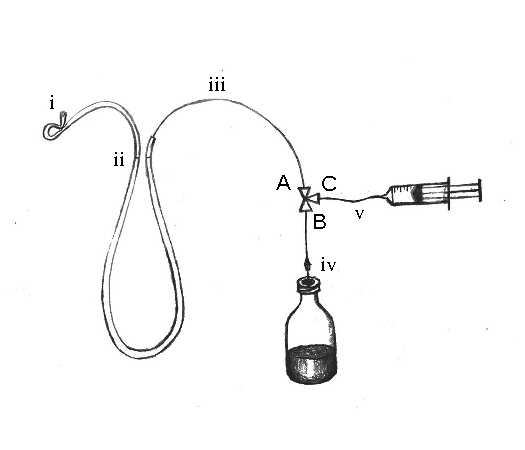
\includegraphics[]{figs/GD_utube.pdf}
  \caption{Sistema experimental para medir el volumen de biogás producido. La línea discontinua indica el manómetro en forma de U; este puede ser sustituido por un manómetro digital.} 
  \label{fig:utube}
\end{figure}

\subsection{Instrucciones paso a paso} 
\label{sec:steps}
\begin{enumerate}
    \item Anotar la temperatura ambiente y presión atmosférica a la que se va a merdir el volumen de biogás.
    \item Sacar las 3 botellas de control de arena de la incubadora y pesarlas para confirmar la consistencia de la balanza. 
      Continuar con las mediciones si los pesos del control son parecidos a los iniciales (teniendo en cuenta la precisión de la balanza). En caso contrario, solucionar el problema antes de continuar con las mediciones (o cambiar de balanza si es necesario).
      Si el problema no se puede solucionar, continua con las mediciones y posteriormente corrige por la desviación de los pesos.\footnote{
        La corrección se realiza substrayendo la diferencia de peso promedio de los controles a todos los pesos realizados en el evento de muestreo. 
        Por ejemplo, si los controles pesan 0.1 gramos más que al inicio del ensayo, el peso de \textit{todas} las botellas en este evento de muestreo se tiene que reducir 0.1 gramos. Realizar este tipo de correciones no es recomendado y tiene que ser la última opción.
      }
    \item Sacar una botella de la incubadora.
    \item Agitar suavemente el contenido de la botella durante 10 segundos para mezclar el contenido y equilibrar el contenido de \ce{CO2} entre la solución y el espacio de cabeza. \textbf{IMPORTANTE: al agitar, evitar que el líquido toque el septo para evitar pérdidas de masa cuando se introduce la aguja, ya que cualquier pérdida de masa representa una fuente de error}.\footnote{Si hay una pérdida de masa por el septo al pinchar el septo con la ajuga anotarlo para poder interpretar los resultados correctamente. Si la pérdida de masa es menospreciable, se puede ignorar el problema. Por otro lado, si el error es notable se tiene que descartar los valores obtenidos de esta botella.}
    \item Pesar la botella y apuntar el peso de la botella antes del venteo.
    \item Ventear el biogás usando una jeringa y medir el volumen de biogás (ver Sección \ref{sec:volmeas}). Evitar que la aguja entre en contacto con el líquido.
    Usar el manómetro (tubo en U, digital) para asegurar que la presión del espacio de cabeza de la botella después del ventear (o al final de cada ciclo) es similar ($\pm3 $ kPa) a la presión atmosférica. 
    
    \item Pesar la botella y apuntar el peso de la botella después del venteo.
    \item Devolver la botella a la incubadora
    \item Repetir el procedimiento para el resto de las botellas

\end{enumerate}

La Fig. \ref{fig:steps} muestra paso a paso las etapas del proceso

\begin{figure}[ht]
  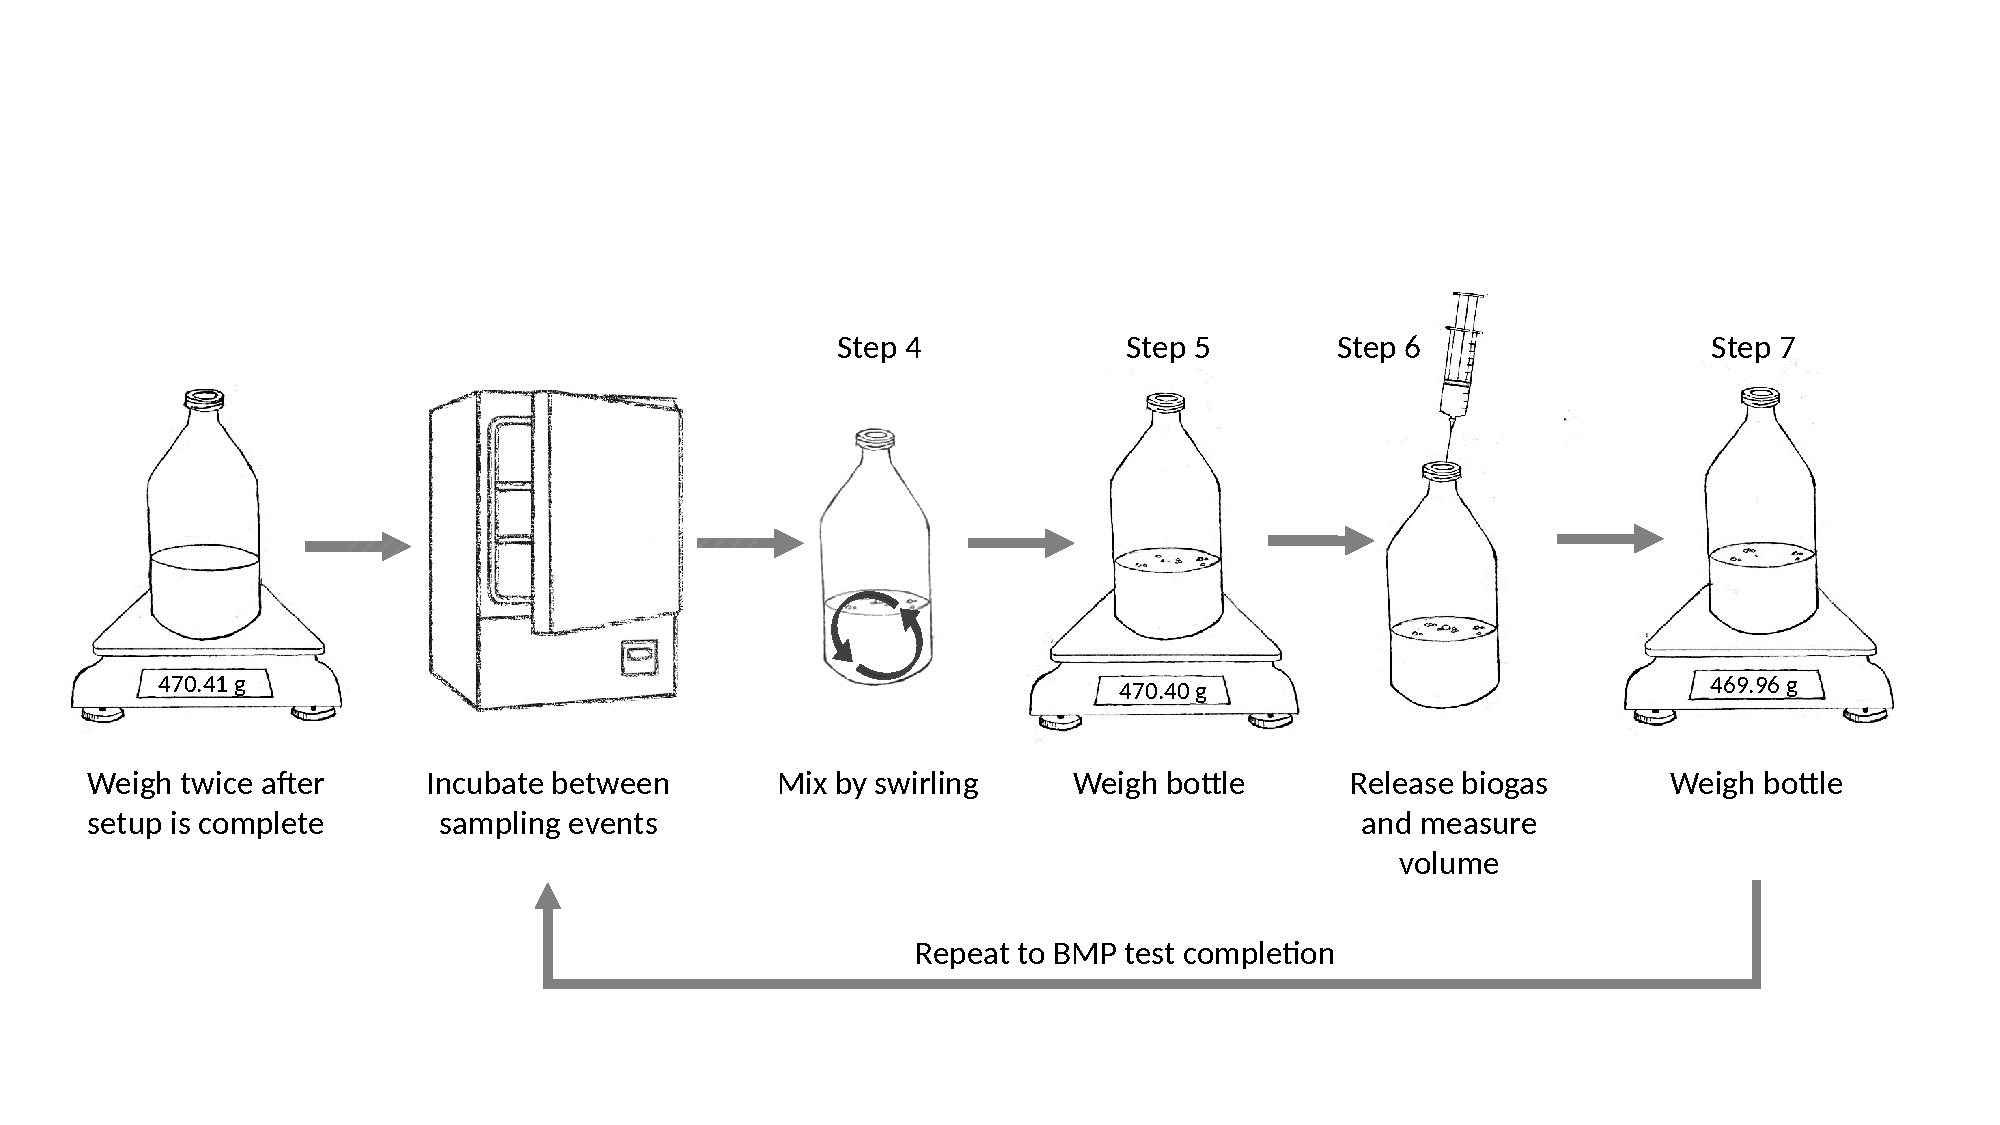
\includegraphics[width=\textwidth]{figs/GD_steps.pdf}
  \caption{The data collection steps required for GD-BMP measurements. Step numbers match those listed in the text, and are repeated for each sampling event. For details on volume measurement (step 6) see Section \ref{sec:volmeas}.}
  \label{fig:steps}
\end{figure}


\section{Método GD-BMP}
El método GD-BMP requiere medir con precisión el volumen de biogás y la pérdida de masa.
Es importante comprobar el método y variaciones del mismo antes de realizar un experimento.
El método se puede verificar con aire.
Para verificar el sistema, introduce \textit{con cuidado} aire dentro de una botella con una jeringa y realiza los pasos descritos anteriormente. 
Calcular la densidad aparente utilizando la pérdida de masa y el volumen de aire eliminado.\footnote{Este volumen es ligeramente inferior al que se piensa que se ha añadido por pequeñas fugas durante el proceso.}
El error de la medición debería ser inferior al 10\% (mejor inferior al 5\%) de la densidad del aire a la temperatura y presión de trabajo.\footnote{La densidad del aire se puede calcular en  \url{https://www.density.co.uk/calculators/density-of-air/} o similares. El efecto de la humedad puede menospreciarse a temperatura ambiente ($\le$ 25$^\circ$C). La densidad del aire seco es 1.20 mg mL$^{-1}$ a 20$^\circ$C y 101.3 kPa, y de 1.19 mg mL$^{-1}$ cuando el aire está saturado con vapor de agua.}

\section{Cálculos}
El documento 204 de esta colección de documentos \citep{BMPdoc204gasdens} explicada detalladamente los cálculos necesarios para el método GD-BMP e incluye un ejemplo. Este documento también está traducido al español.
Los cálculos también se pueden realizar en la aplicacion OBA (online y gratuita)  (\url{https://biotransformers.shinyapps.io/oba1/}) o con el \textit{biogas package} en R (\url{https://cran.r-project.org/package=biogas}) \citep{hafnerSoftwareBiogasResearch2018}.
La validación de los resultados experimentales deben cumplir los criterios mínimos descritos en \citep{BMPdoc100req}.

\bibliography{bib}

\end{document}
